\documentclass[10pt]{beamer}

%load any additional packages

\usepackage[UKenglish]{babel}
\usepackage[utf8]{inputenc} % so we can input characters with accents (e.g. ő)

\usepackage{statsbeamer}
\usepackage{multirow,booktabs}%pacotes para tabelas
\usepackage{subcaption}
\usepackage[font=footnotesize,skip=2pt]{caption}
%\captionsetup[table]{skip=2pt}
\usepackage{ragged2e}
\usepackage{hyperref}
\usepackage{tikz}
\usetikzlibrary{arrows.meta}
\tikzset{%
  >={Latex[width=2mm,length=2mm]},
  % Specifications for style of nodes:
            base/.style = {rectangle, rounded corners, draw=black,
                           minimum width=4cm, minimum height=1cm,
                           text centered, font=\sffamily},
  activityStarts/.style = {base, fill=oxfordblue!30},
       startstop/.style = {base, fill=oxfordblue!30},
    activityRuns/.style = {base, fill=oxfordblue!30},
         process/.style = {base, minimum width=2.5cm, fill=orange!15},
}

\usepackage{graphicx} % ease graphics management
\graphicspath{{figs/}} % define folder with images
\usefonttheme{serif} % change font to allow \textbf{}
\usepackage{charter} % Nicer fonts

\usepackage{cancel}
\usepackage{amsmath,amsthm,amssymb} % for math equations

\usepackage[numbers]{natbib} % richer citation
\usepackage{breakcites} % avoid overfull hbox for long cites

\usepackage{algorithm,algorithmic}                                          % Pseudo-code environment
\usepackage{amsmath,amsfonts,amsthm,amssymb,bm,mathdots,mathtools,bigints}  % Math packages

\usepackage{caption}                        % Tools for customizing the \caption{} command
\usepackage{subcaption}						% Environment to create subcaptions

\captionsetup{singlelinecheck = false, format= hang, justification=raggedright, font=footnotesize, labelsep=space} % ABNT Format for Caption
%% Information (author, title, etc.) %%

\title[Short Title]{% short title for footer
    Separable Least-Mean Squares Beamforming 
    \vspace{0.5cm}
}

\author{Kenneth B. dos A. Benício}

\institute{
        \textit{Department of Teleinformatics Engineering}\\
        \textit{Federal University of Ceará}
        \vspace{0.5cm}
}
\date[Fortaleza, 2021]{% short date for footer
    Fortaleza, 2021
}


%% Content of slides %%
\begin{document}

%% Title slide
{
    \setbeamertemplate{footline}{}
    \setbeamertemplate{headline}{}
    \setbeamercolor{background canvas}{bg=oxfordblue}
    \maketitle
}


%% Contents slide
 \begin{frame}
 \frametitle{Outline}
 \tableofcontents
 \end{frame}

%% Including the slides
\setbeamercovered{transparent}

%% Introduction
\section{Introduction}
\begin{frame}
    \frametitle{\insertsection}
    \begin{itemize}
        \justifying
        \item Comparisons with LMS, NLMS,ATLMS and TLMS.
        \item Convergence Analysis ? 
    \end{itemize}
\end{frame}

%% System Model
\section{System Model}
\begin{frame}
    \frametitle{\insertsection}

\end{frame}

%% Implemented Algorithms
\section{Implemented Algorithms}
\begin{frame}[allowframebreaks]
    \frametitle{\insertsection}
    \begin{figure}
        \centering
        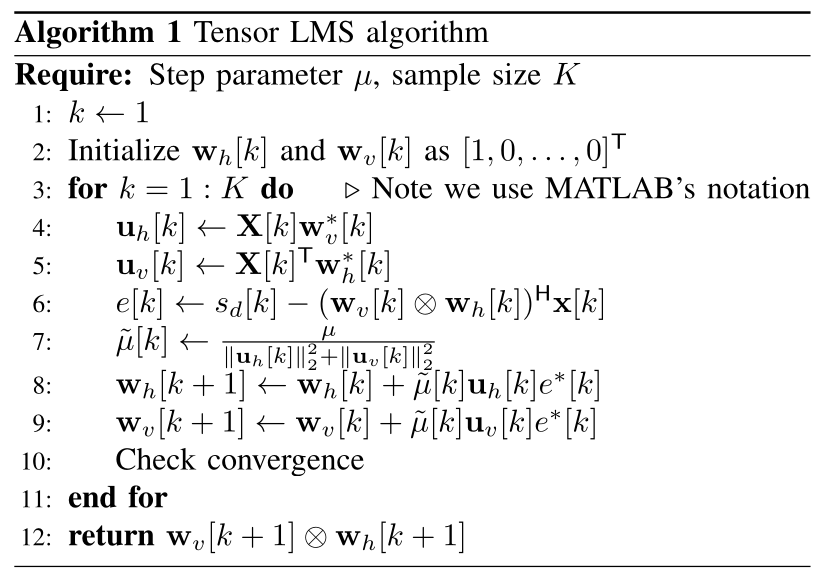
\includegraphics[width=0.90\linewidth]{tlms.png}
        \caption{TLMS algorithm from \cite{ribeiroseparable}.}
        \label{fig:lms_alg} 
    \end{figure}
    \begin{figure}
        \centering
        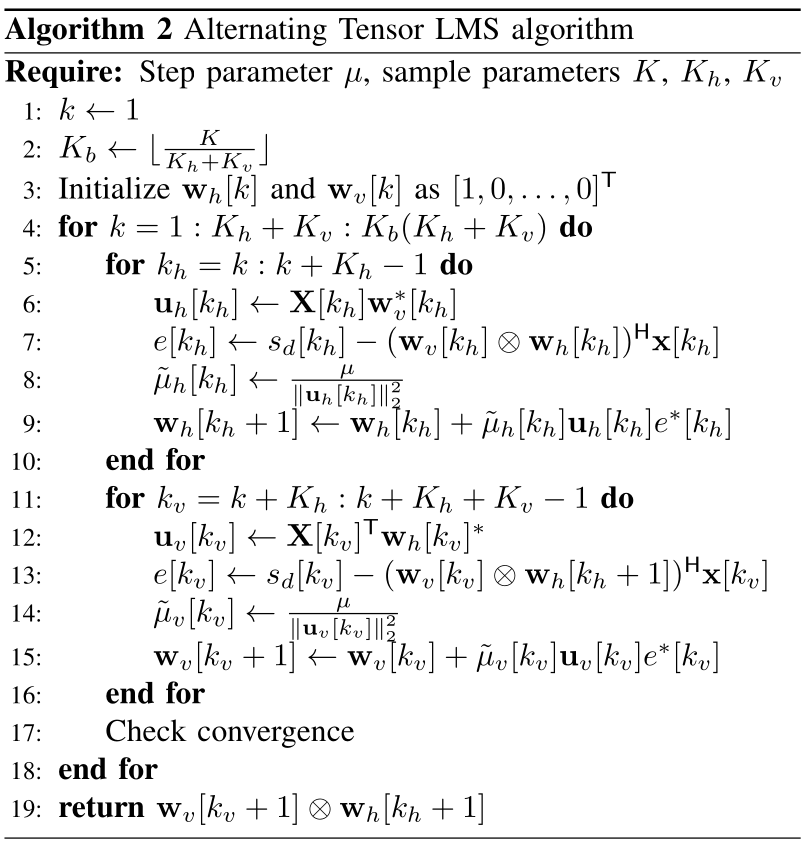
\includegraphics[width=0.60\linewidth]{atlms.png}
        \caption{ATLMS algorithm from \cite{ribeiroseparable}.}
        \label{fig:atlms_alg} 
    \end{figure}
\end{frame}

%% Numerical Results
\section{Numerical Results}
\begin{frame}[allowframebreaks]
    \frametitle{\insertsection}
    \begin{figure}
        \centering
        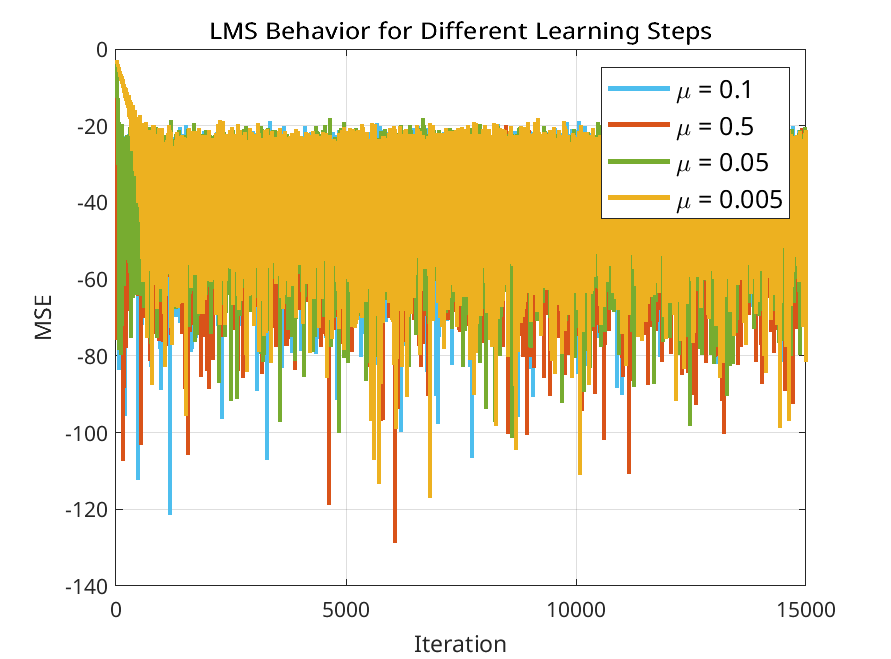
\includegraphics[width=0.90\linewidth]{lms_mse.png}
        \caption{Monter Carlo Experiment with 2500 runs for LMS algorithm.}
        \label{fig:lms} 
    \end{figure}
    \begin{figure}
        \centering
        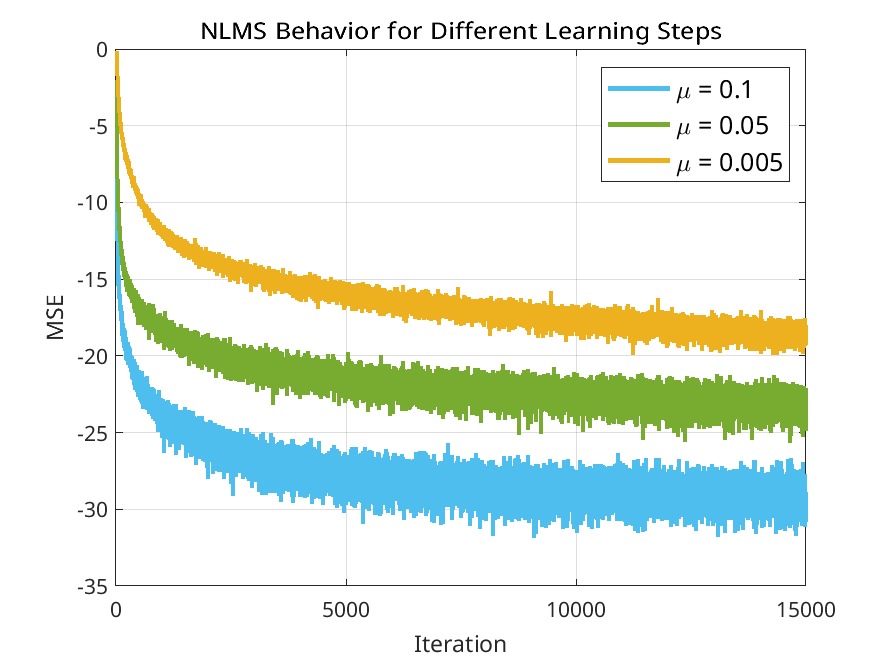
\includegraphics[width=0.90\linewidth]{nlms_mse.png}
        \caption{Monter Carlo Experiment with 2500 runs for LMS algorithm.}
        \label{fig:nlms} 
    \end{figure}
    \begin{figure}
        \centering
        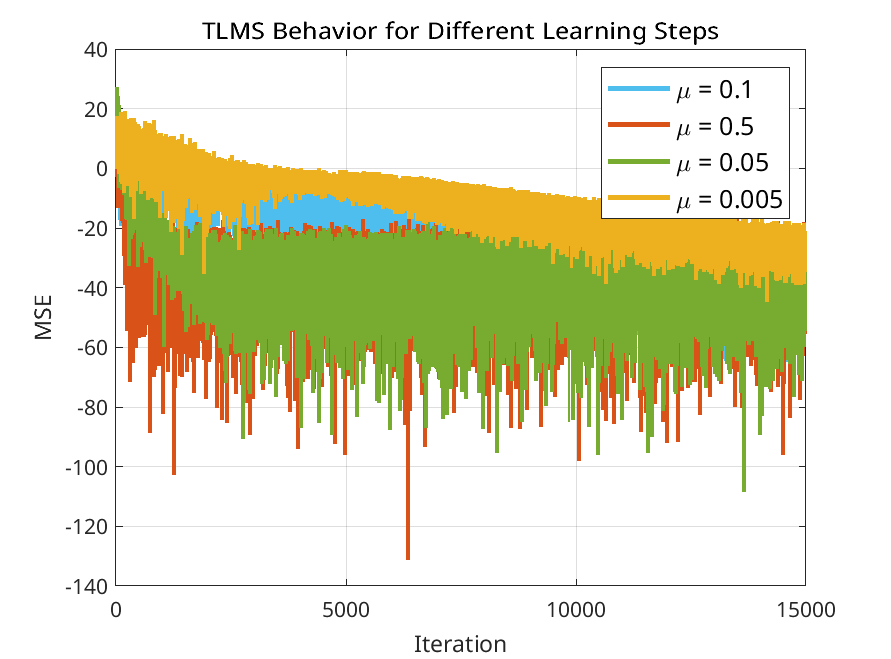
\includegraphics[width=0.90\linewidth]{tlms_mse.png}
        \caption{Monter Carlo Experiment with 2500 runs for LMS algorithm.}
        \label{fig:tlms} 
    \end{figure}
    \begin{figure}
        \centering
        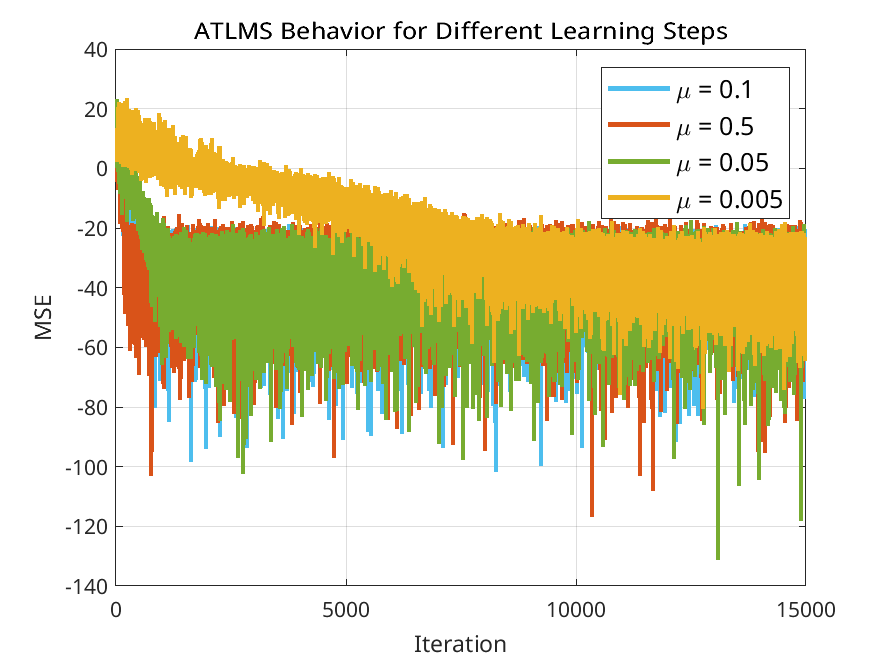
\includegraphics[width=0.90\linewidth]{atlms_mse.png}
        \caption{Monter Carlo Experiment with 2500 runs for LMS algorithm.}
        \label{fig:atlms} 
    \end{figure}
    \begin{figure}
        \centering
        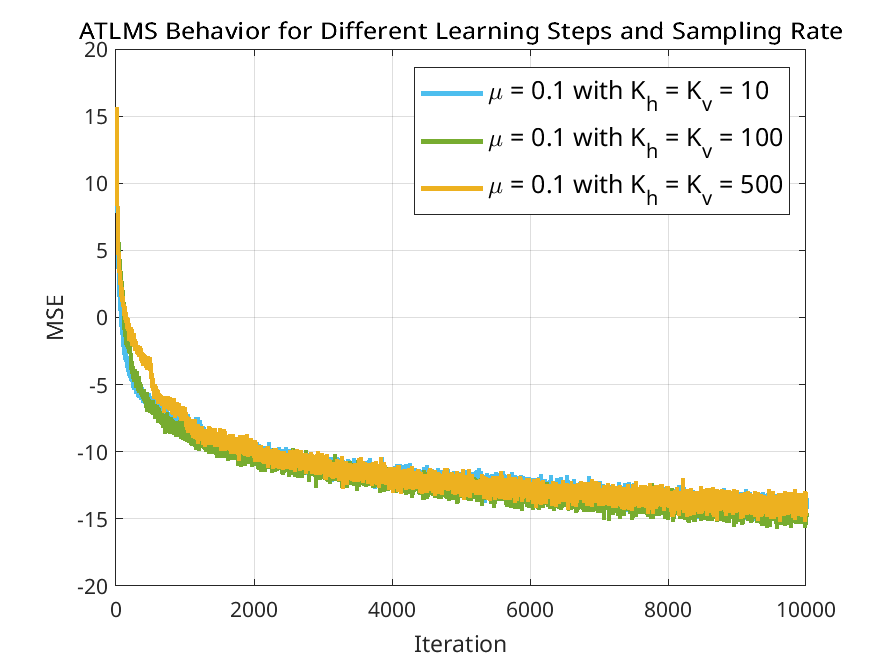
\includegraphics[width=0.90\linewidth]{atlms_sampling.png}
        \caption{Monter Carlo Experiment with 2500 runs for the ATLMS with different sampling intervals.}
        \label{fig:atlms_sampling} 
    \end{figure}
    \begin{figure}
        \centering
        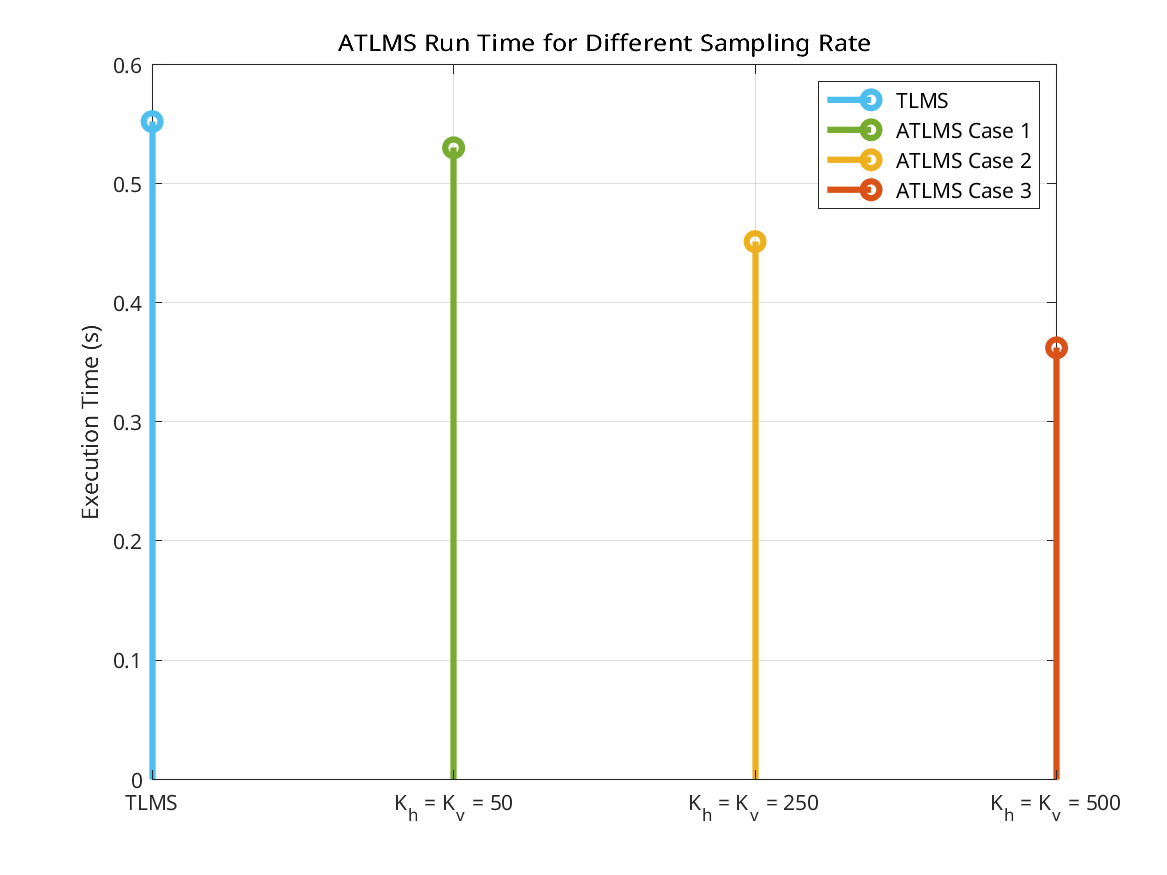
\includegraphics[width=0.90\linewidth]{atlms_time.png}
        \caption{Run time process for ATLMS with different sampling intervals.}
        \label{fig:atlms_time} 
    \end{figure}
\end{frame}

%% References
\section{References}
\begin{frame} 
    \frametitle{\insertsection}
    \bibliographystyle{ieeetr}
    \bibliography{references}
\end{frame}

%% End of Presentation
\begin{frame}
    \begin{center}
        \Huge Thank you for your presence!
    \end{center}
\end{frame}

\end{document}